\chapter{MOTION PLANNING}
\label{ch:Motion planning}
In this chapter we explain the solution to plan the trajectory of the end effector in order to unwound the string from the pivots.

\section{Involute of a circle}
Let's start talking about the involute of a circle. This one was discovered in 1673 by Christiaan Huygens, a Dutch mathematician and physicist. In his work titled "Horologium oscillatorium sive de motu pendulorum ad horologia aptato demonstrationes geometricae", he focused upon the theories about the motion of pendulum. He was interested in making clocks for ships at sea. Finding a clock which would keep accurate time at sea was a major problem and many years were spent looking for a solution. This issue was of vital importance since if GMT was known from a clock then, since local time could be easily computed from the sun, longitude could be easily computed.  He introduced there the concept of involute or evolvent of the curve and he used the circle involute in his first pendulum clock in an attempt to force the pendulum to swing in the path of a cycloid \cite{mccleary2013geometry}. 

%The problem was that it was not possible to have a normal oscillating pendulum in these clocks as the rocking of ships on sea would alter the pendulum movements. Therefore there had to be a way for clocks without pendulums to show correct time. He introduced there the concept of involute or evolvent of the curve and he used the circle involute in his first pendulum clock in an attempt to force the pendulum to swing in the path of a cycloid. 

In differential geometry, the involute is defined as a curve that is obtained by attaching an imaginary string and winding or unwinding it tautly on the given curve. The locus of the free end of this attached taut string is known as an involute or an evolvent  \cite{mccleary2013geometry}.

The involute of a given curve can also be defined as a line segment that is tangent to the curve on one end, while the other end traces out the involute. This line segment is wound or reversely unwound along with the continuous variation in the length of line segment by a certain amount. The curve so traced by free end is called an involute  \cite{mccleary2013geometry}.

In the case of this project, we have to unwound the string from circular pivots, the solution is thus the involute of a circle. This is the curve traced by the free end of a thread unwound from a circle in such a way that the thread is always tight and tangential to the circle. More practically, it is the curve traced by a hand unwinding a wire reel held in the other hand.

In this curve, all the normals are tangent to a fixed circle. Conversely, if an involute of a circle turns around the centre of the generating circle, every tangent to the circle remains always normal to the involute.

Figure~\ref{fig:involute} below shows how the involute of a circle looks like:

\begin{figure}[htbp]
	\centering
	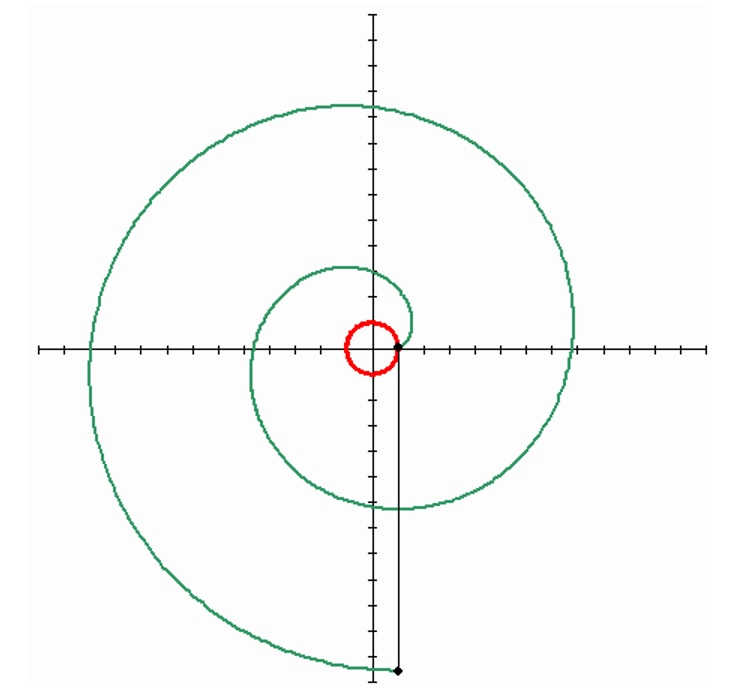
\includegraphics[height=70mm]{chapters/figures/motion_planning/involute.jpg}
	\caption{Involute of a circle.}
	\label{fig:involute}
\end{figure}

Its parametric equations in the Cartesian coordinates are:
\begin{equation*}
\begin{split}
x = a \cdot (cos(t) + t \cdot sin(t)) \\ 
y = a \cdot (sin(t) - t \cdot cos(t))
\end{split}
\end{equation*}

Where \textit{a} is the radius of the circle and \textit{t} is the angle in radians.

We noticed that the involute of a circle has a very similar shape to the Archimedean spiral.

\section{Archimedean spiral}
The Archimedean spiral is the asymptotic curve to the involute of a circle for large values of the angle \textit{t}. It also is its pedal with respect to the center \cite{weisstein2003pedal}.

The pedal curve results from the orthogonal projection of a fixed point on the tangent lines of a given curve. The pedal of a curve with respect to a point O (or with pole O) is the locus of the feet of the lines passing by O perpendicular to the tangents to the curve \cite{weisstein2003pedal}. 

The Archimedean spiral, also known as arithmetic spiral,  is a spiral named after the 3rd century BC Greek mathematician Archimedes. It is the trajectory of a point moving uniformly (with a constant speed) on a straight line of a plane, this line turning itself uniformly (rotating with constant angular velocity) around one of its points \cite{sloane}. It has the property that any ray from the origin intersects successive turnings of the spiral in points with a constant separation distance, hence the name "arithmetic spiral" \cite{holland1957archimedes}.

The Archimedean spiral has two arms, one for angle $t > 0\textdegree$ and one for $t < 0\textdegree$. The two arms are smoothly connected at the origin. Only one arm is shown in Figure~\ref{fig:spiral}. Taking the mirror image of this arm across the y-axis will yield the other arm.

\begin{figure}[htbp]
	\centering
	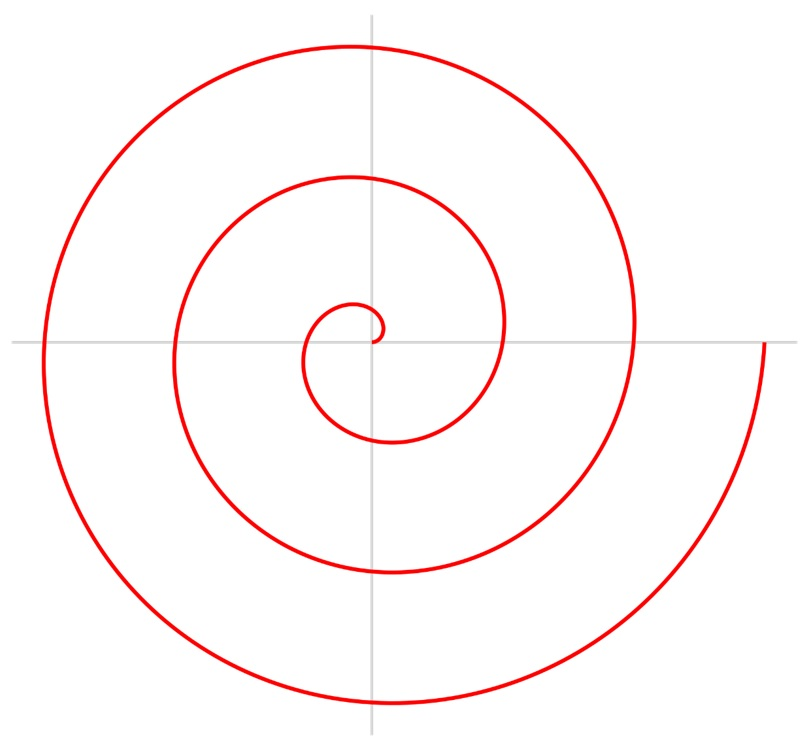
\includegraphics[height=70mm]{chapters/figures/motion_planning/spiral.jpg}
	\caption{Archimedean spiral.}
	\label{fig:spiral}
\end{figure}

Its parametric equation is the one shown below:
\begin{equation*}
\begin{split}
x = r \cdot t \cdot cos(t) \\ 
y = r \cdot t \cdot sin(t)
\end{split}
\end{equation*}

Where \textit{r} is the radius of the spiral and \textit{t} is the angle in radians.

Let's now compare the differences between the involute of a circle and the Archimedean spiral.

\section{Comparison between involute of a circle and Archimedean spiral}
As told before, involute of a circle and Archimedean spiral have very similar shapes. In this section we compare them and talk about the differences. Figure~\ref{fig:comparison} below shows the difference in both shapes.\newpage
\begin{figure}[h!]
	\centering
	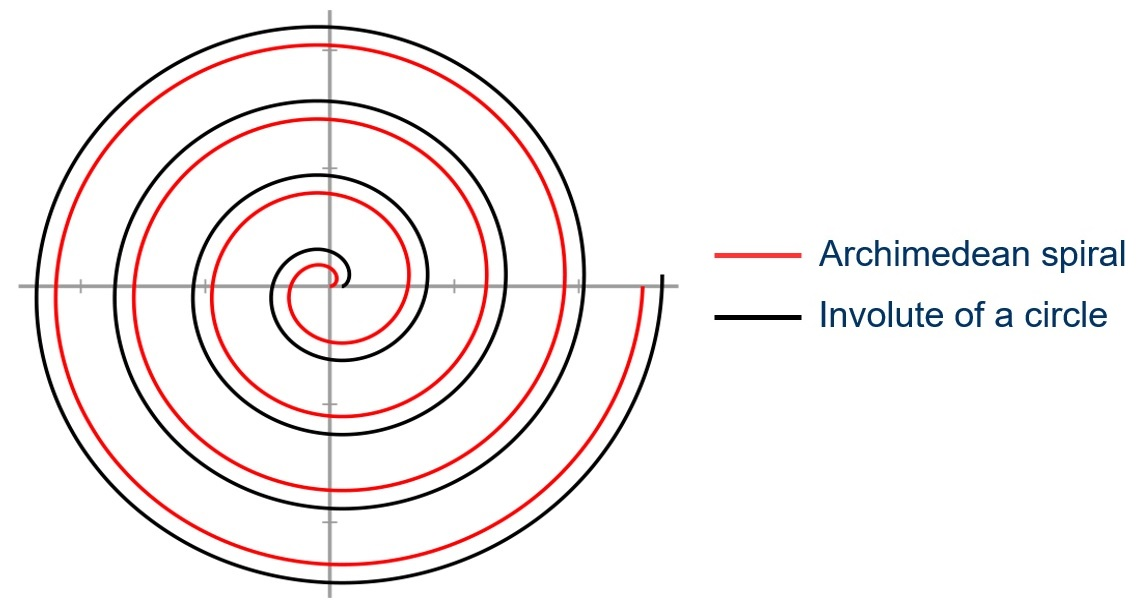
\includegraphics[height=80mm]{chapters/figures/motion_planning/comparison.jpg}
	\caption{Comparison between involute of a circle and Archimedean spiral.}
	\label{fig:comparison}
\end{figure}

Archimedean spiral is represented in red and involute of a cirlce in black. Both radius are the same, 1 unit. They seem to have the same progress as the angle increases but let's see the real differences in Table~\ref{table:comparison} below.

\begin{table}[!ht]
\begin{center}
\begin{tabular}{l|*{2}{c}r}
	                  & Archimedean spiral & Involute of a circle \\
	\hline
	Angles            & $0 \leq t \leq 8\pi$ & $0 \leq t \leq \frac{17\pi}{2}$ \\
	\hline
	Initial position  & x = 0 & x = 1 \\
	                  & y = 0 & y = 0 \\
	\hline
	Final position    & x = 25.12 & x = 26.7 \\
	                  & y = 0     & y = 1    \\
	\hline
	Equation          & $x = r \cdot t \cdot cos(t)$ & $x = a \cdot (cos(t) + t \cdot sin(t))$ \\
	                  & $y = r \cdot t \cdot sin(t)$ & $y = a \cdot (sin(t) - t \cdot cos(t))$ \\
\end{tabular}
\end{center}
\caption{Comparison between involute of a circle and Archimedean spiral.}
\label{table:comparison}
\end{table}

Let's comment the values on the table. 

If we look at Figure~\ref{fig:comparison}, both curves seem to finish almost at the same angle. However, if we look to the values on the table, we see that involute of a circle finishes $\frac{\pi}{2}$ later than the Archimidean spiral.

Concerning initial and final positions, we appreciate that the difference at the beginning is 1 unit, but at the end the difference is almost 1.6 units. We can say thus that in 4 turns, the difference between involute of a circle and Archimedean spiral increases around 0.6 units, this is 0.6/4 = 0.15 units in each turn.

Finally, if we compare both equations, we see that the equation for Armchimidean spiral is much more easy to understand and to apply than the one for involute of a circle.

As the radius of our pivots is small (0.4 mm) and the length of the string (34 cm) and distance between pivots (4.25 cm) limit the number of turns (to 5 or 6 maximum), Archimidean spiral and involute will have very similar results. So, as the equation for Archimidean spiral is easier to apply, we decide to use this one in this project in order to untie the string from the circular pivots.

Let's now show and explain the algorithm we came up with to open the string-envelope.
